\documentclass[11pt]{article}
\usepackage[margin=1in]{geometry}
\usepackage[T1]{fontenc}
\usepackage[utf8]{inputenc}
\usepackage{lmodern}
\usepackage{microtype}
\usepackage[table]{xcolor}
\usepackage{amsmath,amssymb,amsfonts,mathtools,bm}
\IfFileExists{physics.sty}{%
  \usepackage{physics}%
}{%
  % Portable subset used by this project when the optional physics package
  % is not installed in the local TeX distribution.
  \NewDocumentCommand{\pdv}{o m m}{%
    \IfNoValueTF{##1}{\frac{\partial ##2}{\partial ##3}}%
    {\frac{\partial^{##1} ##2}{\partial ##3^{##1}}}%
  }
  \NewDocumentCommand{\dv}{o m m}{%
    \IfNoValueTF{##1}{\frac{\mathrm{d} ##2}{\mathrm{d} ##3}}%
    {\frac{\mathrm{d}^{##1} ##2}{\mathrm{d} ##3^{##1}}}%
  }
  \providecommand{\dd}{\mathop{}\!\mathrm{d}}
  \providecommand{\grad}{\nabla}
  \providecommand{\abs}[1]{\left\lvert ##1\right\rvert}
  \providecommand{\norm}[1]{\left\lVert ##1\right\rVert}
  \providecommand{\ket}[1]{\left\lvert ##1\right\rangle}
  \providecommand{\bra}[1]{\left\langle ##1\right\rvert}
}
\usepackage{booktabs,array,longtable,tabularx}
\usepackage{hyperref}
\usepackage{enumitem}
\usepackage{fancyhdr}
\usepackage{titlesec}
\usepackage{tcolorbox}
\usepackage{ragged2e}
\usepackage{setspace}
\IfFileExists{siunitx.sty}{%
  \usepackage{siunitx}%
}{%
  % Minimal text-safe fallback for the small number of \SI and \si calls in
  % this repository. Full siunitx formatting is used when available.
  \providecommand{\si}[1]{\ensuremath{\mathrm{##1}}}
  \providecommand{\SI}[2]{\ensuremath{##1\,\mathrm{##2}}}
}
\hypersetup{colorlinks=true, linkcolor=blue!50!black, urlcolor=blue!50!black, citecolor=blue!50!black}
\definecolor{TitleBlue}{HTML}{163A5F}
\definecolor{AccentTeal}{HTML}{2D6F73}
\definecolor{SoftBlue}{HTML}{EAF3F8}
\definecolor{SoftTeal}{HTML}{EDF8F6}
\definecolor{SoftGray}{HTML}{F5F7FA}
\definecolor{RuleGray}{HTML}{D7DEE8}
\pagestyle{fancy}
\fancyhf{}
\lhead{RadiationEffects\_proj2}
\rhead{Technical Notes}
\cfoot{\thepage}
\setlength{\headheight}{14pt}
\setlength{\parskip}{0.5em}
\setlength{\parindent}{0pt}
\onehalfspacing
\numberwithin{equation}{section}
\titleformat{\section}{\Large\bfseries\color{TitleBlue}}{\thesection}{0.6em}{}
\titleformat{\subsection}{\large\bfseries\color{AccentTeal}}{\thesubsection}{0.6em}{}
\titleformat{\subsubsection}{\normalsize\bfseries\color{TitleBlue}}{\thesubsubsection}{0.6em}{}
\newtcolorbox{overviewbox}{colback=SoftBlue,colframe=TitleBlue,boxrule=0.8pt,arc=2mm,left=3mm,right=3mm,top=2mm,bottom=2mm}
\newtcolorbox{physicsbox}{colback=SoftTeal,colframe=AccentTeal,boxrule=0.8pt,arc=2mm,left=3mm,right=3mm,top=2mm,bottom=2mm}
\newtcolorbox{notebox}{colback=SoftGray,colframe=AccentTeal,boxrule=0.6pt,arc=2mm,left=3mm,right=3mm,top=2mm,bottom=2mm}
\newcommand{\DocTitle}[3]{%
\begin{center}
{\LARGE \bfseries \color{TitleBlue} #1}\\[0.5em]
{\large \color{AccentTeal} #2}\\[0.8em]
{\normalsize #3}
\end{center}
\vspace{0.5em}}
\newenvironment{symtable}{\rowcolors{2}{SoftGray}{white}\begin{longtable}{>{\RaggedRight\arraybackslash}p{0.18\textwidth} >{\RaggedRight\arraybackslash}p{0.25\textwidth} >{\RaggedRight\arraybackslash}p{0.47\textwidth}}\toprule \textbf{Symbol / acronym} & \textbf{Name} & \textbf{Meaning in this document} \\ \midrule\endfirsthead\toprule \textbf{Symbol / acronym} & \textbf{Name} & \textbf{Meaning in this document} \\ \midrule\endhead}{\bottomrule\end{longtable}}


\newcommand{\ProjectTOC}{%
\vspace{0.6em}
{\hypersetup{linkcolor=TitleBlue,urlcolor=TitleBlue,citecolor=TitleBlue}\tableofcontents}
\vspace{1.0em}}

\newcommand{\SymbolsAcronymsSection}{%
\section*{Symbols and acronyms used in this document}%
\addcontentsline{toc}{section}{Symbols and acronyms used in this document}}

\newcommand{\rvec}{\bm{r}}
\newcommand{\qvec}{\bm{q}}
\newcommand{\nvec}{\bm{n}}
\newcommand{\xvec}{\bm{x}}
\newcommand{\kB}{k_{\mathrm{B}}}
\newcommand{\qp}{\mathrm{qp}}
\newcommand{\JJ}{\mathrm{JJ}}
\newcommand{\mfp}{\Lambda}
\allowdisplaybreaks

\usepackage{tikz}
\usetikzlibrary{arrows.meta,positioning,shapes.geometric,calc,decorations.pathmorphing}

\newcommand{\Om}{\Omega}
\newcommand{\Osub}{\Omega_{\mathrm{sub}}}
\newcommand{\Oox}{\Omega_{\mathrm{ox}}}
\newcommand{\Osc}{\Omega_{\mathrm{sc}}}
\newcommand{\Ojj}{\Omega_{\mathrm{JJ}}}
\newcommand{\Gint}{\Gamma_{\mathrm{int}}}
\newcommand{\Evec}{\bm{E}}
\newcommand{\Jvec}{\bm{J}}
\newcommand{\Avec}{\bm{A}}
\newcommand{\vvec}{\bm{v}}
\newcommand{\x}{\bm{x}}
\newcommand{\nvecb}{\bm{n}}
\newcommand{\gradxy}{\nabla_{xy}}
\newcommand{\divxy}{\nabla_{xy}\cdot}
\newcommand{\phiE}{\phi}
\newcommand{\DeltaSC}{\Delta}
\newcommand{\Tc}{T_{\mathrm{c}}}
\newcommand{\Ns}{n_{\mathrm{s}}}
\newcommand{\ncp}{n_{\mathrm{cp}}}
\newcommand{\nqp}{n_{\mathrm{qp}}}
\newcommand{\xqp}{x_{\mathrm{qp}}}
\newcommand{\Nzero}{N_0}
\newcommand{\Jqp}{\bm{J}_{\mathrm{qp}}}
\newcommand{\Js}{\bm{J}_{\mathrm{s}}}
\newcommand{\Jtot}{\bm{J}_{\mathrm{tot}}}
\newcommand{\muq}{\mu_{\mathrm{q}}}
\newcommand{\mustar}{\mu^*}
\newcommand{\muchem}{\mu_{\mathrm{chem}}}
\newcommand{\muec}{\mu_{\mathrm{ec}}}
\newcommand{\Dqp}{D_{\mathrm{qp}}}
\newcommand{\Gqp}{G_{\mathrm{qp}}}
\newcommand{\Rqp}{R_{\mathrm{qp}}}
\newcommand{\tauqp}{\tau_{\mathrm{qp}}}
\newcommand{\tautrap}{\tau_{\mathrm{trap}}}
\newcommand{\tautun}{\tau_{\mathrm{tun}}}
\newcommand{\GammaQP}{\Gamma_{\mathrm{qp}}}
\newcommand{\GammaPB}{\Gamma_{\mathrm{pb}}}
\newcommand{\GammaT}{\Gamma_{\mathrm{trap}}}
\newcommand{\Iqp}{I_{\mathrm{qp}}}
\newcommand{\Ic}{I_{\mathrm{c}}}
\newcommand{\Ijj}{I_{\mathrm{J}}}
\newcommand{\VJ}{V_{\mathrm{J}}}
\newcommand{\CJ}{C_{\mathrm{J}}}
\newcommand{\EJ}{E_{\mathrm{J}}}
\newcommand{\EC}{E_{\mathrm{C}}}
\newcommand{\ngate}{n_{\mathrm{g}}}
\newcommand{\Qoff}{Q_{\mathrm{off}}}
\newcommand{\Qis}{Q_{\mathrm{is}}}
\newcommand{\Cmat}{\bm{C}}
\newcommand{\Vvec}{\bm{V}}
\newcommand{\Qvec}{\bm{Q}}
\newcommand{\Geh}{G_{eh}}
\newcommand{\Reh}{R_{eh}}
\newcommand{\Dch}{D_{\mathrm{ch}}}
\newcommand{\Gch}{G_{\mathrm{ch}}}
\newcommand{\Rch}{R_{\mathrm{ch}}}
\newcommand{\Nt}{N_{\mathrm{t}}}
\newcommand{\ft}{f_{\mathrm{t}}}
\newcommand{\rhooff}{\rho_{\mathrm{off}}}
\newcommand{\wpot}{\psi}
\newcommand{\Tph}{T_{\mathrm{ph}}}
\newcommand{\Te}{T_{\mathrm{e}}}
\newcommand{\Vt}{V_T}
\newcommand{\hbarTwoe}{\frac{\hbar}{2e}}
\newcommand{\Phizero}{\Phi_0}

\rhead{Module 5 superconductivity}
\begin{document}

\DocTitle{Module 5 Superconductivity Extension: Carrier Transport, Quasiparticle Poisoning, Offset Charge, and Josephson-Device Response}{How the preexisting drift-diffusion carrier-transport module changes in the superconducting region}{Physics note for RadiationEffects\_proj2}

\begin{overviewbox}
\textbf{Purpose.} Module 5 originally converted electrostatic, defect, and thermal fields into semiconductor carrier transport: mobile electrons and holes obey drift-diffusion equations with generation, recombination, mobility degradation, and current output. This superconductivity extension explains what changes when the radiation-effects problem is moved to cryogenic superconducting-device operation. The main change is that the relevant mobile charge carriers are no longer only ordinary conduction-band electrons and valence-band holes. The device may contain frozen-out semiconductor substrate carriers, trapped charges in dielectrics, superconducting condensate current, quasiparticle diffusion in superconducting films, quasiparticle tunneling across Josephson junctions, and radiation-induced offset-charge motion. This note derives these pieces in a textbook style and translates them into Module 5 modeling requirements.
\end{overviewbox}

\ProjectTOC

\SymbolsAcronymsSection
\begin{symtable}
Module 5 & Carrier-transport module & Existing module that evolves mobile charge carriers and computes electrical response. \\
SC & Superconducting & Condensed state below a critical temperature with zero DC resistance in ideal equilibrium and an excitation gap. \\
QP & Quasiparticle & Broken-Cooper-pair excitation in a superconductor. \\
DD & Drift-diffusion & Semiconductor transport model for mobile electrons and holes. \\
SRH & Shockley-Read-Hall & Trap-assisted recombination through localized defect states. \\
JJ & Josephson junction & Weak link between superconductors; supports phase-dependent supercurrent and quasiparticle tunneling. \\
TLS & Two-level system & Defect-like microscopic degree of freedom that can fluctuate and couple to electric fields or qubits. \\
CP & Cooper pair & Bound pair of electrons forming the superconducting condensate. \\
PBP & Pair-breaking phonon & Phonon with energy sufficient to break a Cooper pair, approximately \(\hbar\omega\ge 2\Delta\). \\
\(\x\) & Position & Spatial coordinate in the 2D or 3D device. \\
\(t\) & Time & Time coordinate. \\
\(q,e\) & Elementary charge magnitude & Positive scalar charge magnitude. In superconductivity notation, the Cooper-pair charge magnitude is \(2e\). \\
\(\phiE\) & Electrostatic potential & Scalar potential from Module 2. \\
\(\Evec\) & Electric field & \(\Evec=-\nabla\phiE\). \\
\(n,p\) & Semiconductor carriers & Mobile electron and hole concentrations in the baseline Module 5 model. \\
\(\Geh\) & Electron-hole generation & Generation rate of ordinary mobile electron-hole pairs in a semiconductor or dielectric. \\
\(\Reh\) & Electron-hole recombination & Recombination rate of ordinary mobile electron-hole pairs. \\
\(\DeltaSC\) & Superconducting gap & Minimum energy of one quasiparticle excitation. \\
\(\Tc\) & Critical temperature & Temperature below which superconductivity appears. \\
\(\Ns\) & Superfluid density & Density participating in condensate response. \\
\(\ncp\) & Cooper-pair density & Number density of Cooper pairs; electron superfluid density is approximately \(2\ncp\). \\
\(\theta\) & Condensate phase & Phase of the superconducting order parameter. \\
\(\Avec\) & Magnetic vector potential & Vector potential entering gauge-invariant condensate momentum. \\
\(\Js\) & Supercurrent density & Current density carried by the superconducting condensate. \\
\(\Jqp\) & Quasiparticle current density & Current density carried by quasiparticle excitations. \\
\(\Jtot\) & Total current density & Sum of condensate, quasiparticle, and possibly displacement or normal currents. \\
\(\nqp\) & Quasiparticle density & Number of QPs per unit superconducting-film volume. \\
\(\xqp\) & Normalized QP density & Common dimensionless measure, roughly \(\nqp/(2N_0\Delta)\). \\
\(\Nzero\) & Single-spin density of states & Normal-state density of states at the Fermi level. \\
\(\Dqp\) & QP diffusivity & Effective diffusion coefficient for QPs in a superconducting film. \\
\(\Gqp\) & QP generation rate & Rate at which QPs are produced by pair-breaking phonons, photons, radiation, or injection. \\
\(\Rqp\) & QP recombination coefficient & Coefficient for approximate QP recombination loss. \\
\(\tauqp\) & QP lifetime & Effective time scale for QP removal by recombination, trapping, or escape. \\
\(\tautrap\) & Trap time & Characteristic time for QP trapping/removal. \\
\(\GammaQP\) & QP tunneling rate & Rate of QP tunneling across a Josephson junction or weak link. \\
\(\GammaPB\) & Pair-breaking generation rate & QP generation rate caused by pair-breaking phonons. \\
\(\muchem\) & Chemical potential & Thermodynamic chemical potential of particles. \\
\(\muec\) & Electrochemical potential & Chemical plus electrostatic potential energy. \\
\(\mustar\) & Charge-imbalance potential & Nonequilibrium quasiparticle charge-mode potential. \\
\(\Ic\) & Critical current & Maximum Josephson supercurrent in the zero-voltage branch. \\
\(\delta\) & Junction phase difference & Gauge-invariant phase difference across a Josephson junction. \\
\(\Ijj\) & Josephson current & \(\Ijj=\Ic\sin\delta\). \\
\(\VJ\) & Junction voltage & Voltage across a Josephson junction. \\
\(\CJ\) & Junction capacitance & Capacitance across the tunnel barrier. \\
\(\EJ\) & Josephson energy & \(\EJ=\hbar\Ic/(2e)\). \\
\(\EC\) & Charging energy & Island charging scale, often \(\EC=e^2/(2C_\Sigma)\). \\
\(\Qoff\) & Offset charge & Effective environmental charge coupled capacitively to a superconducting island. \\
\(\ngate\) & Dimensionless gate charge & \(\ngate=Q_{\mathrm{g}}/(2e)\), with radiation/traps contributing to \(Q_{\mathrm{g}}\). \\
\(\Nt\) & Trap density & Density of localized charge traps. \\
\(\ft\) & Trap occupation & Occupation probability of a trap. \\
\(\rhooff\) & Offset-charge density & Radiation-induced charge density that couples electrostatically to superconducting islands. \\
\(\wpot\) & Weighting potential & Solution of an auxiliary electrostatic problem used to compute induced island charge. \\
\(\Tph\) & Phonon temperature & Effective phonon-bath temperature from Module 4, when local equilibrium is meaningful. \\
\(\Te\) & Electron temperature & Effective electronic temperature, if the electronic subsystem is thermalized. \\
\end{symtable}

\section{What Module 5 did before superconductivity}

Baseline Module 5 is a semiconductor drift-diffusion carrier-transport module. Its unknowns are mobile electron and hole concentrations,
\begin{equation}
 n(\x,t),\qquad p(\x,t),
\end{equation}
which are driven by the electrostatic potential \(\phiE\), electric field \(\Evec=-\nabla\phiE\), temperature \(T\), and defect populations \(C_j\) provided by Modules 2, 3, and 4. In a two-dimensional reduced model, the usual continuity equations are
\begin{align}
\pdv{n}{t} + \nabla\cdot \bm{\Gamma}_n &= G_n-R_n, \\
\pdv{p}{t} + \nabla\cdot \bm{\Gamma}_p &= G_p-R_p,
\end{align}
where \(\bm{\Gamma}_n\) and \(\bm{\Gamma}_p\) are particle fluxes. The conventional electrical currents are
\begin{align}
 \Jvec_n &= q\mu_n n\Evec + qD_n\nabla n,\\
 \Jvec_p &= q\mu_p p\Evec - qD_p\nabla p,\\
 \Jvec &= \Jvec_n+\Jvec_p.
\end{align}
Defects enter through mobility reduction, generation/recombination, and space-charge feedback:
\begin{align}
\mu_n &= \mu_{n0}(T) F_n(C_1,C_2,\ldots),\\
\mu_p &= \mu_{p0}(T) F_p(C_1,C_2,\ldots),\\
R &\supset R_{\mathrm{SRH}}(n,p,N_t,E_t,T),\\
\rho &= q(p-n+N_D^+-N_A^-+\rho_{\mathrm{def}}/q).
\end{align}
Thus the baseline causal chain is
\begin{equation}
\boxed{\phiE,\Evec,T,C_j \longrightarrow \mu_n,\mu_p,G,R \longrightarrow n,p,\Jvec \longrightarrow y_{\mathrm{device}}.}
\end{equation}

\begin{physicsbox}
\textbf{Baseline Module 5 intuition.} Radiation changes semiconductor transport because it creates mobile carriers, creates traps, changes recombination, changes mobility, and changes the electric field. That picture is correct for ordinary semiconductor devices. It is not sufficient for a superconducting qubit or superconducting sensor because the electrically relevant carriers include a condensate and quasiparticles, not merely ordinary electrons and holes.
\end{physicsbox}

\section{The first conceptual change below the superconducting transition}

A superconducting device is a hybrid object. It may contain a silicon or sapphire substrate, oxide or dielectric layers, native interfaces, normal-metal structures, superconducting films, and Josephson junction tunnel barriers. Cooling the device below \(\Tc\) does not make every region superconducting. Instead, the material regions must be separated:
\begin{equation}
\Om = \Osub \cup \Oox \cup \Osc \cup \Ojj \cup \Omega_{\mathrm{normal}}.
\end{equation}
Each region carries charge differently.

\begin{center}
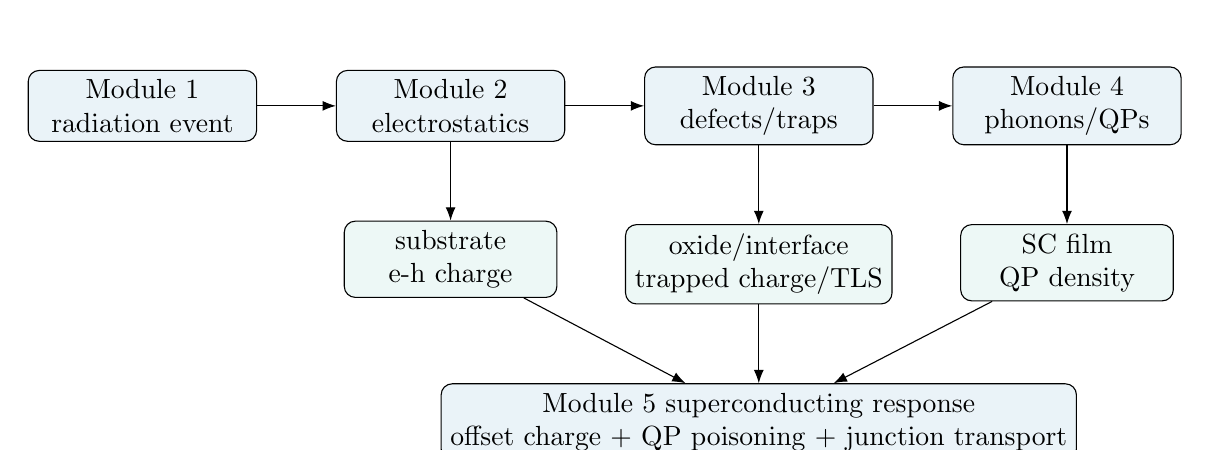
\begin{tikzpicture}[node distance=0.6cm,>=Latex]
\tikzstyle{blk}=[draw,rounded corners,align=center,minimum width=2.9cm,minimum height=0.85cm,fill=SoftBlue]
\tikzstyle{smallblk}=[draw,rounded corners,align=center,minimum width=2.7cm,minimum height=0.8cm,fill=SoftTeal]
\node[blk] (m1) {Module 1\\radiation event};
\node[blk,right=1.0cm of m1] (m2) {Module 2\\electrostatics};
\node[blk,right=1.0cm of m2] (m3) {Module 3\\defects/traps};
\node[blk,right=1.0cm of m3] (m4) {Module 4\\phonons/QPs};
\node[smallblk,below=1.0cm of m2] (sub) {substrate\\e-h charge};
\node[smallblk,below=1.0cm of m3] (trap) {oxide/interface\\trapped charge/TLS};
\node[smallblk,below=1.0cm of m4] (qp) {SC film\\QP density};
\node[blk,below=1.0cm of trap] (m5) {Module 5 superconducting response\\offset charge + QP poisoning + junction transport};
\draw[->] (m1)--(m2);
\draw[->] (m2)--(m3);
\draw[->] (m3)--(m4);
\draw[->] (m2)--(sub);
\draw[->] (m3)--(trap);
\draw[->] (m4)--(qp);
\draw[->] (sub)--(m5);
\draw[->] (trap)--(m5);
\draw[->] (qp)--(m5);
\end{tikzpicture}
\end{center}

The most important warning is this:
\begin{equation}
\boxed{\text{Do not replace } n,p \text{ by one superconducting carrier density.}}
\end{equation}
The superconducting condensate, quasiparticles, ordinary semiconductor carriers, trapped charges, and tunnel-barrier defects are different physical populations with different time scales and different equations.

\subsection{Which carrier populations remain relevant?}

In the superconducting extension of Module 5, the old variables \(n,p\) are not simply deleted. Instead, they become material-dependent and event-dependent:
\begin{align}
 n_{\mathrm{sub}}(\x,t),\;p_{\mathrm{sub}}(\x,t) &\quad \text{transient radiation-generated substrate carriers},\\
 \ft(\x,t) &\quad \text{trap/TLS occupations in oxide, interfaces, and junction barriers},\\
 \theta(\x,t),\;\Ns(\x,T) &\quad \text{condensate phase and superfluid density},\\
 \nqp(\x,t) &\quad \text{quasiparticle density in superconducting films},\\
 \delta(t) &\quad \text{Josephson phase difference across a junction},\\
 \Qoff(t) &\quad \text{radiation-induced offset charge coupled to islands}.
\end{align}
For a superconducting qubit application, the primary Module 5 output may no longer be a semiconductor leakage current. It may be a set of poisoning and charge-noise metrics:
\begin{equation}
\boxed{\nqp(\x,t),\quad \GammaQP(t),\quad \Qoff(t),\quad \delta\omega_q(t),\quad \Gamma_1^{\mathrm{qp}}(t),\quad \text{parity-switching rate}.}
\end{equation}

\section{Semiconductor carriers at cryogenic temperature: freeze-out and radiation bursts}

Start with the part of the device that is not superconducting: the substrate or dielectric. If the substrate is silicon at millikelvin temperature, thermally generated mobile carrier densities are usually strongly suppressed. A standard nondegenerate semiconductor estimate is
\begin{equation}
 n_i(T) \propto T^{3/2}\exp\left[-\frac{E_g}{2\kB T}\right].
\end{equation}
At cryogenic temperature, this equilibrium density is negligible for a large-gap semiconductor. Donors and acceptors may also freeze out, because the thermal energy is too small to ionize dopants efficiently. Thus the baseline steady drift-diffusion background often collapses to
\begin{equation}
 n_{\mathrm{eq}}\approx 0,\qquad p_{\mathrm{eq}}\approx 0
\end{equation}
for an insulating substrate or depleted semiconductor region.

But radiation changes this. A single ionizing event can create many electron-hole pairs and high-energy phonons. Therefore the correct cryogenic substrate equation is not a steady room-temperature drift-diffusion problem. It is an event-driven transient transport and trapping problem:
\begin{align}
\pdv{n_{\mathrm{sub}}}{t}+\nabla\cdot\bm{\Gamma}_{n,\mathrm{sub}} &= G_{eh}^{\mathrm{rad}}-R_{eh}^{\mathrm{sub}}-R_{n\to t},\\
\pdv{p_{\mathrm{sub}}}{t}+\nabla\cdot\bm{\Gamma}_{p,\mathrm{sub}} &= G_{eh}^{\mathrm{rad}}-R_{eh}^{\mathrm{sub}}-R_{p\to t},\\
\pdv{\ft}{t} &= c_n n_{\mathrm{sub}}(1-\ft)-e_n\ft-c_p p_{\mathrm{sub}}\ft+e_p(1-\ft).
\end{align}
Here \(\ft\) is a trap occupation, \(c_n,c_p\) are capture coefficients, and \(e_n,e_p\) are emission coefficients. At millikelvin temperature, thermally activated emission may be extremely slow. In reduced Module 5 language, this means trap occupancy can store the memory of a radiation event.

\subsection{Drift and diffusion are still possible, but the parameters change}

For transient radiation-generated substrate charge, the old drift-diffusion flux forms can still be used as a reduced model:
\begin{align}
\bm{\Gamma}_{n,\mathrm{sub}} &= -\mu_n n_{\mathrm{sub}}\Evec-D_n\nabla n_{\mathrm{sub}},\\
\bm{\Gamma}_{p,\mathrm{sub}} &= +\mu_p p_{\mathrm{sub}}\Evec-D_p\nabla p_{\mathrm{sub}}.
\end{align}
However, the cryogenic parameter regime is different:
\begin{align}
\mu_{n,p}(T,C_j) &\quad \text{may increase from reduced phonon scattering,}\\
\mu_{n,p}(T,C_j) &\quad \text{may decrease from impurity, interface, and defect scattering,}\\
D_{n,p} &= \mu_{n,p}\frac{\kB T_{\mathrm{carrier}}}{q} \quad \text{only when carriers are locally thermalized.}
\end{align}
The Einstein relation is not automatic after an energetic radiation event. If the carrier distribution is nonthermal, the diffusion coefficient should be treated as an effective transport coefficient or derived from a kinetic calculation.

\begin{notebox}
\textbf{Modeling decision for this project.} For a first superconducting Module 5 extension, it is reasonable to keep a reduced transient drift-diffusion equation in the substrate/dielectric only as a charge-collection and trapped-charge model. It should not be interpreted as ordinary steady semiconductor device operation at room temperature.
\end{notebox}

\section{Superconducting current is not ordinary drift-diffusion}

In a superconducting film, the low-energy charged fluid is the condensate. A useful order parameter is
\begin{equation}
\Psi(\x,t)=\sqrt{\ncp(\x,t)}e^{i\theta(\x,t)},
\end{equation}
where \(\ncp\) is Cooper-pair density and \(\theta\) is phase. The gauge-invariant condensate momentum is
\begin{equation}
\bm{p}_{\mathrm{s}}=\hbar\nabla\theta-2e\Avec.
\end{equation}
The condensate velocity is
\begin{equation}
\bm{v}_{\mathrm{s}}=\frac{1}{2m^*}\left(\hbar\nabla\theta-2e\Avec\right),
\end{equation}
where \(2m^*\) is the approximate Cooper-pair mass. Since each Cooper pair has charge \(-2e\), the supercurrent density is
\begin{equation}
\Js = -2e\ncp\bm{v}_{\mathrm{s}}
= -\frac{e\ncp}{m^*}\left(\hbar\nabla\theta-2e\Avec\right).
\label{eq:supercurrent}
\end{equation}
Depending on sign convention for electron charge and phase, the sign may be written differently. The invariant statement is that the supercurrent is proportional to the gauge-invariant phase gradient.

This is not a drift-diffusion law. It does not say
\begin{equation}
\Js = \sigma\Evec - qD\nabla n.
\end{equation}
In an ideal DC superconducting state, a static electric field inside a bulk superconductor is screened and the electrochemical potential is constant. Sustained DC current is carried by phase stiffness, not by resistive drift in an electric field.

\subsection{Continuity equation for condensate charge}

The condensate charge density is approximately
\begin{equation}
\rho_s=-2e\ncp.
\end{equation}
If condensate density changes, charge conservation gives
\begin{equation}
\pdv{\rho_s}{t}+\nabla\cdot\Js = S_{\mathrm{pair}},
\end{equation}
where \(S_{\mathrm{pair}}\) represents conversion between condensate pairs and quasiparticles. In equilibrium and far from pair breaking, \(S_{\mathrm{pair}}\approx 0\) and \(\ncp\) is effectively fixed by temperature and material properties. For most Module 5 superconducting-device calculations, one should not evolve \(\ncp\) as a free drift-diffusion carrier density. Instead, use material properties \(\Delta(T,C_j)\), \(\Tc(C_j)\), kinetic inductance, and junction parameters.

\subsection{Kinetic inductance as the transport output of the condensate}

The condensate has inertia. A changing current therefore stores kinetic energy. The kinetic-energy density of the condensate is
\begin{equation}
 u_{\mathrm{kin}}=\frac{1}{2}(2m^*)\ncp v_s^2.
\end{equation}
Because \(\Js=-2e\ncp \bm{v}_s\),
\begin{equation}
 u_{\mathrm{kin}}=\frac{m^*}{4e^2\ncp}J_s^2.
\end{equation}
This motivates a kinetic inductance. In a thin superconducting wire or film, reduced \(\ncp\) or increased disorder increases kinetic inductance. Radiation-induced disorder from Module 3 and QP population from Module 4 can therefore feed Module 5 by changing inductive response even without ordinary DC resistance.

\section{Quasiparticle transport in superconducting films}

A quasiparticle is an excitation above the superconducting ground state. It is not the same object as a normal-state electron, but at the reduced modeling level one often evolves the quasiparticle density \(\nqp\). The simplest spatial equation is a diffusion-reaction equation,
\begin{equation}
\pdv{\nqp}{t} = \nabla\cdot(\Dqp\nabla\nqp)+\Gqp-\Rqp\nqp^2-\frac{\nqp-\nqp^{\mathrm{eq}}}{\tautrap}+S_{\mathrm{inj}}.
\label{eq:nqp_diffusion}
\end{equation}
The terms have direct physical meanings:
\begin{align}
\nabla\cdot(\Dqp\nabla\nqp) &\quad \text{spatial spreading of QPs in the superconducting film},\\
\Gqp &\quad \text{generation by pair-breaking phonons, photons, radiation, or injection},\\
\Rqp\nqp^2 &\quad \text{two-QP recombination into a Cooper pair plus phonon energy},\\
(\nqp-\nqp^{\mathrm{eq}})/\tautrap &\quad \text{removal by traps, gap-engineered sinks, or escape},\\
S_{\mathrm{inj}} &\quad \text{intentional or parasitic injection from leads or junctions}.
\end{align}

The equilibrium density at low temperature is exponentially small. A common BCS low-temperature estimate is
\begin{equation}
\nqp^{\mathrm{eq}}(T) \approx 2\Nzero\sqrt{2\pi \kB T\DeltaSC}\exp\left(-\frac{\DeltaSC}{\kB T}\right),
\label{eq:nqp_eq}
\end{equation}
where \(\Nzero\) is the single-spin normal-state density of states at the Fermi level. This exponential factor is why even small nonequilibrium sources can dominate over equilibrium QPs.

\subsection{Why quasiparticle transport is Module 5, not only Module 4}

Module 4 treats energy flow: phonons, pair breaking, recombination energy, and heat. Module 5 treats electrical response. Quasiparticles are an overlap variable because they are both excitations carrying energy and mobile charged degrees of freedom that affect device response. The clean separation is
\begin{align}
\text{Module 4:} \quad & \text{where does deposited energy go?}\\
\text{Module 5:} \quad & \text{how do the resulting QPs and charges change electrical response?}
\end{align}
Thus \(\nqp\) may be computed in Module 4 and then consumed in Module 5, or it may be part of a coupled Module 5 response model. In either case, Module 5 needs \(\nqp\) to compute junction poisoning, parity switching, conductance, and qubit relaxation.

\subsection{Normalized quasiparticle density}

A useful dimensionless QP density is
\begin{equation}
\xqp = \frac{\nqp}{2\Nzero\DeltaSC}.
\label{eq:xqp}
\end{equation}
The denominator is approximately the density of Cooper-pair-scale electronic states near the gap. In superconducting-qubit literature, small \(\xqp\) can still produce measurable relaxation and parity switching because junction tunneling is sensitive to QPs near the gap edge.

\section{Quasiparticle current and charge imbalance}

Equation \eqref{eq:nqp_diffusion} tracks QP number, not necessarily charge current. In superconductors, quasiparticles are coherent mixtures of electron-like and hole-like excitations. A quasiparticle at energy \(E\) has BCS coherence amplitudes \(u_E\) and \(v_E\), and its effective charge expectation is roughly
\begin{equation}
q_E = -e\left(u_E^2-v_E^2\right).
\end{equation}
Near the gap edge, electron-like and hole-like character can nearly cancel. Therefore a QP density gradient does not automatically imply the same electrical current as an ordinary electron density gradient.

A reduced charge-imbalance description introduces a nonequilibrium quasiparticle chemical-potential-like variable \(\mustar\). Then a linear transport form is
\begin{equation}
\Jqp \approx -\sigma_{\mathrm{qp}}\nabla\left(\frac{\mustar}{e}\right),
\label{eq:qp_current}
\end{equation}
with a relaxation equation
\begin{equation}
\pdv{\mustar}{t}=D_Q\nabla^2\mustar-\frac{\mustar}{\tau_Q}+S_Q.
\end{equation}
Here \(\tau_Q\) is a charge-imbalance relaxation time and \(S_Q\) represents injection or radiation-generated imbalance. This is a higher-fidelity transport model than simply equating QP density diffusion with electrical current.

\begin{notebox}
\textbf{Practical reduced model.} For the first RadiationEffects\_proj2 superconducting Module 5 extension, use \(\nqp\) as the main QP transport state and compute poisoning metrics from it. Add \(\mustar\) only if the project specifically needs nonequilibrium charge-imbalance voltages or quasiparticle charge current.
\end{notebox}

\section{Josephson junction transport replaces ordinary drift current across the weak link}

The most important electrical nonlinearity in a superconducting qubit is often the Josephson junction. A tunnel junction has two kinds of current:
\begin{equation}
I = I_{\mathrm{s}} + I_{\mathrm{qp}} + I_C + I_{\mathrm{noise}}.
\end{equation}
The supercurrent branch is
\begin{equation}
I_{\mathrm{s}}=\Ic\sin\delta,
\label{eq:josephson_current}
\end{equation}
where \(\delta\) is the gauge-invariant phase difference. The phase and voltage are related by
\begin{equation}
\VJ = \hbarTwoe\pdv{\delta}{t}.
\label{eq:josephson_voltage}
\end{equation}
The capacitive current is
\begin{equation}
I_C=\CJ\pdv{\VJ}{t}.
\end{equation}
A resistively and capacitively shunted reduced junction equation is therefore
\begin{equation}
\CJ\hbarTwoe\pdv[2]{\delta}{t}+\frac{1}{R_{\mathrm{qp}}}\hbarTwoe\pdv{\delta}{t}+\Ic\sin\delta=I_{\mathrm{bias}}+I_{\mathrm{noise}},
\label{eq:rcsj}
\end{equation}
where \(R_{\mathrm{qp}}\) should be interpreted carefully: it is not an ordinary room-temperature semiconductor resistance. It represents dissipative quasiparticle tunneling and any effective subgap conductance.

\subsection{Josephson energy and charging energy}

The Josephson energy follows from integrating the supercurrent with respect to phase:
\begin{equation}
E_J(\delta) = -\EJ\cos\delta,\qquad \EJ=\frac{\hbar\Ic}{2e}.
\end{equation}
A superconducting island also stores electrostatic energy. If its total capacitance is \(C_\Sigma\), the charging energy scale is
\begin{equation}
\EC=\frac{e^2}{2C_\Sigma}.
\end{equation}
For an island with integer Cooper-pair number \(N\) and dimensionless offset charge \(\ngate\), the charging term is
\begin{equation}
H_C = 4\EC (N-\ngate)^2,
\qquad
\ngate = \frac{Q_g+\Qoff}{2e}.
\label{eq:charging}
\end{equation}
This equation is central to the radiation problem. Radiation-induced trapped charge does not have to conduct through the junction to affect the qubit. It can shift \(\Qoff\), thereby shifting \(\ngate\), thereby changing device frequency or parity-sensitive observables.

\section{Quasiparticle tunneling and poisoning}

Quasiparticles in a superconducting electrode can tunnel across a Josephson junction. This tunneling can change the island parity, dissipate energy, and relax a qubit. A reduced local model writes the QP tunneling rate as proportional to the QP density near the junction:
\begin{equation}
\GammaQP(t) \approx \gamma_{\mathrm{tun}}\,\overline{\xqp}_{\mathrm{JJ}}(t),
\label{eq:gamma_qp_reduced}
\end{equation}
where \(\overline{\xqp}_{\mathrm{JJ}}\) is a junction-neighborhood average of \(\xqp\), and \(\gamma_{\mathrm{tun}}\) is a calibrated coefficient depending on junction conductance, gap, matrix elements, and qubit mode. A more explicit averaging definition is
\begin{equation}
\overline{\xqp}_{\mathrm{JJ}}(t)=\frac{\int_{\Osc} W_{\mathrm{JJ}}(\x)\xqp(\x,t)\,d\Om}{\int_{\Osc} W_{\mathrm{JJ}}(\x)\,d\Om},
\end{equation}
where \(W_{\mathrm{JJ}}\) weights the electrode regions that efficiently tunnel into the junction.

For qubit relaxation modeling, a reduced proportionality is often sufficient:
\begin{equation}
\Gamma_1^{\mathrm{qp}}(t) \equiv \frac{1}{T_{1,\mathrm{qp}}(t)} \approx A_q \overline{\xqp}_{\mathrm{JJ}}(t),
\label{eq:t1_qp}
\end{equation}
where \(A_q\) is a device-dependent coefficient. This is not a substitute for microscopic tunneling theory, but it is the correct reduced response architecture for RadiationEffects\_proj2: radiation source \(\rightarrow\) phonons/QPs \(\rightarrow\) local QP density near junction \(\rightarrow\) device-level degradation metric.

\subsection{Pair-breaking generation source from Module 4}

Module 4 supplies a pair-breaking phonon field or a reduced pair-breaking source. In Module 5 this enters as
\begin{equation}
\Gqp(\x,t)=\GammaPB(\x,t)+G_{\mathrm{IR}}(\x,t)+G_{\mathrm{inj}}(\x,t),
\end{equation}
where \(\GammaPB\) is due to high-energy phonons with \(\hbar\omega\ge 2\Delta\), \(G_{\mathrm{IR}}\) is due to stray photons/infrared radiation, and \(G_{\mathrm{inj}}\) represents junction or lead injection.

A reduced energy-to-QP conversion relation is
\begin{equation}
N_{\mathrm{qp,gen}} \approx \eta_{\mathrm{qp}}\frac{E_{\mathrm{abs,sc}}}{\DeltaSC},
\end{equation}
where \(E_{\mathrm{abs,sc}}\) is radiation-induced energy absorbed into the superconducting film and \(\eta_{\mathrm{qp}}\) is an efficiency factor. The factor is not universal because some energy downconverts into subgap phonons or escapes before breaking pairs.

\section{Offset charge from radiation-generated carriers and traps}

Radiation can create electron-hole pairs in the substrate and trapped charge in dielectrics or interfaces. Even if this charge never becomes a conduction current, it can capacitively shift a superconducting island. Module 2 computes electrostatics; Module 3 computes trap populations; Module 5 converts them into device response.

Let \(\rhooff(\x,t)\) be the radiation-induced charge density outside the superconducting island. The induced charge on island \(a\) can be computed using a weighting potential \(\wpot_a\). Define \(\wpot_a\) by the auxiliary electrostatic problem
\begin{align}
\nabla\cdot(\epsilon\nabla \wpot_a)&=0 \quad \text{in dielectric/substrate regions},\\
\wpot_a&=1 \quad \text{on island } a,\\
\wpot_a&=0 \quad \text{on other conductors},\\
\nvecb\cdot\epsilon\nabla\wpot_a&=0 \quad \text{on insulating outer boundaries, if appropriate}.
\end{align}
Then the induced offset charge is
\begin{equation}
\Qoff,a(t)=\int_{\Om\setminus \Omega_{\mathrm{metal}}} \rhooff(\x,t)\wpot_a(\x)\,d\Om.
\label{eq:weighting_offset}
\end{equation}
This is the carrier-transport consequence of radiation-generated charge. The charge distribution comes from substrate carrier motion and trap occupation; the device response comes from the induced \(\Qoff\).

\subsection{Trap occupation as a stochastic or continuum variable}

For a trap species with charge \(q_t\), density \(\Nt(\x)\), and occupation \(\ft(\x,t)\), the trapped-charge density is
\begin{equation}
\rho_t(\x,t)=q_t\Nt(\x)\ft(\x,t).
\end{equation}
Substitution into Eq. \eqref{eq:weighting_offset} gives
\begin{equation}
\Qoff,a(t)=\sum_t\int q_t\Nt^{(t)}(\x)\ft^{(t)}(\x,t)\wpot_a(\x)\,d\Om.
\end{equation}
For a single microscopic trap switching between two occupations, the contribution is a random telegraph signal,
\begin{equation}
\Delta Q_{a}=q_t\wpot_a(\x_t),
\end{equation}
where \(\x_t\) is the trap location. This is the bridge between Module 3 TLS/trap physics and Module 5 charge-noise response.

\begin{physicsbox}
\textbf{Key intuition.} In a superconducting qubit, a radiation-created charge does not need to become a measured current to matter. It can simply move or become trapped near a high-participation electrostatic region, changing offset charge and therefore changing the qubit Hamiltonian.
\end{physicsbox}

\section{Capacitance-matrix formulation for superconducting islands}

A superconducting circuit with multiple islands is naturally described by a capacitance matrix. If island voltages are collected in \(\Vvec\), the island charges satisfy
\begin{equation}
\Qvec = \Cmat \Vvec + \Qvec_{\mathrm{off}}.
\end{equation}
The electrostatic energy is
\begin{equation}
U_C=\frac{1}{2}\left(\Qvec-\Qvec_{\mathrm{off}}\right)^T \Cmat^{-1}\left(\Qvec-\Qvec_{\mathrm{off}}\right).
\label{eq:cap_matrix_energy}
\end{equation}
For a single island, this reduces to the familiar charging-energy expression. For a multi-island device, radiation-induced charge can shift several islands with correlations determined by the weighting potentials and capacitance matrix.

This provides a clean Module 5 output map:
\begin{equation}
\boxed{\rhooff(\x,t) \longrightarrow \Qvec_{\mathrm{off}}(t) \longrightarrow U_C(t) \longrightarrow \delta\omega_q(t),\;\delta\ngate(t),\;\text{charge-noise metric}.}
\end{equation}

\section{How defects alter superconducting carrier response}

Module 3 supplies defect fields. In ordinary Module 5, those defects modify electron and hole mobility and SRH recombination. In the superconducting extension, defects modify a different set of response parameters:
\begin{align}
C_j(\x,t) &\longrightarrow \DeltaSC(\x,t),\; \Tc(\x,t),\; \Ns(\x,t),\\
C_j(\x,t) &\longrightarrow \Dqp(\x,t),\; \Rqp(\x,t),\; \tautrap(\x,t),\\
C_j(\x,t) &\longrightarrow \Ic(t),\; R_N(t),\; \CJ(t),\; \GammaQP(t),\\
C_j(\x,t) &\longrightarrow \Nt(\x,t),\; \ft(\x,t),\; \Qoff(t).
\end{align}
Here \(R_N\) is the normal-state junction resistance or effective tunnel resistance. The exact maps are material-specific. A reduced phenomenological version may be
\begin{align}
\DeltaSC(\x,t) &= \Delta_0\left[1-a_\Delta \sum_j C_j(\x,t)\right]_+,\\
\Dqp(\x,t) &= \frac{1}{3}v_{\mathrm{qp}}(\Delta,T)\ell_{\mathrm{qp}}(\x,t),\\
\ell_{\mathrm{qp}}^{-1}(\x,t) &= \ell_0^{-1}+\sum_j \alpha_j C_j(\x,t),\\
\tautrap^{-1}(\x,t) &= \tau_{0}^{-1}+\sum_j \beta_j C_j(\x,t).
\end{align}
These equations should be treated as reduced closure laws, not universal constants. Their value is that they preserve the causal structure of the multiphysics model.

\section{Radiation event chain for superconducting Module 5}

For a superconducting qubit-like device, a useful event chain is
\begin{equation}
\boxed{E_{\mathrm{dep}} \rightarrow \{e\text{-}h\;\text{pairs},\;\text{phonons},\;\text{traps}\} \rightarrow \{\Qoff,\;\nqp\} \rightarrow \{\Gamma_1^{\mathrm{qp}},\;\Gamma_{\mathrm{parity}},\;\delta\omega_q\}.}
\end{equation}
This chain has two main branches.

\subsection{Charge branch}

The charge branch is
\begin{align}
E_{\mathrm{dep}} &\longrightarrow G_{eh}^{\mathrm{rad}}(\x,t),\\
G_{eh}^{\mathrm{rad}} &\longrightarrow n_{\mathrm{sub}},p_{\mathrm{sub}},\ft,\\
n_{\mathrm{sub}},p_{\mathrm{sub}},\ft &\longrightarrow \rhooff(\x,t),\\
\rhooff &\longrightarrow \Qoff(t),\\
\Qoff &\longrightarrow \ngate(t),\;\delta\omega_q(t),\;\text{charge-noise observables}.
\end{align}
A reduced generation estimate is
\begin{equation}
G_{eh}^{\mathrm{rad}}(\x,t)=\eta_{eh}\frac{\dot q_{\mathrm{dep}}(\x,t)}{\varepsilon_{eh}},
\end{equation}
where \(\varepsilon_{eh}\) is the mean energy per electron-hole pair in the substrate material and \(\eta_{eh}\) is an efficiency factor.

\subsection{Quasiparticle branch}

The quasiparticle branch is
\begin{align}
E_{\mathrm{dep}} &\longrightarrow \text{high-energy phonons},\\
\text{high-energy phonons} &\longrightarrow \GammaPB(\x,t),\\
\GammaPB &\longrightarrow \nqp(\x,t),\\
\nqp &\longrightarrow \GammaQP(t),\;\Gamma_1^{\mathrm{qp}}(t),\;\text{parity switching}.
\end{align}
A reduced QP equation with Module 4 source input is
\begin{equation}
\pdv{\nqp}{t}=\nabla\cdot(\Dqp\nabla\nqp)+\eta_{\mathrm{pb}}\frac{P_{2\Delta}(\x,t)}{\DeltaSC}-\Rqp\nqp^2-\frac{\nqp}{\tautrap},
\end{equation}
where \(P_{2\Delta}\) is the power density in phonons energetic enough to break pairs.

\section{Boundary and interface conditions}

Superconducting Module 5 needs different boundary conditions for each carrier type.

\subsection{Substrate charge boundaries}

For transient substrate carriers,
\begin{equation}
\bm{\Gamma}_{n,p}\cdot\nvecb = 0
\end{equation}
represents insulating boundaries. A collecting electrode or recombination surface can be modeled by
\begin{equation}
\bm{\Gamma}_{n}\cdot\nvecb = S_n(n-n_{\mathrm{eq}}),\qquad
\bm{\Gamma}_{p}\cdot\nvecb = S_p(p-p_{\mathrm{eq}}),
\end{equation}
where \(S_n,S_p\) are surface loss velocities. At cryogenic temperature these should often be interpreted as trapping/collection rates, not thermal equilibrium recombination speeds.

\subsection{Quasiparticle film boundaries}

For QP diffusion in a superconducting film,
\begin{equation}
-\Dqp\nabla\nqp\cdot\nvecb = 0
\end{equation}
represents reflecting boundaries. A QP trap or sink can be modeled by
\begin{equation}
-\Dqp\nabla\nqp\cdot\nvecb = S_{\mathrm{qp}}\left(\nqp-\nqp^{\mathrm{trap}}\right).
\end{equation}
At a material interface, continuity of QP current and appropriate transmission/trapping conditions are needed:
\begin{align}
\nqp^{(1)} &\leftrightarrow \nqp^{(2)} \quad \text{through an interface conductance or transmission law},\\
-D_1\nabla\nqp^{(1)}\cdot\nvecb_1 &= G_{12}\left(\nqp^{(1)}-\alpha_{12}\nqp^{(2)}\right).
\end{align}

\subsection{Junction coupling boundary}

Near a Josephson junction, QP density should feed a local tunneling sink/source:
\begin{equation}
-D_{\mathrm{L}}\nabla\nqp^{\mathrm{L}}\cdot\nvecb = S_{\mathrm{tun}}\left(\nqp^{\mathrm{L}}-\nqp^{\mathrm{R}}\right)+S_{\mathrm{relax}}\nqp^{\mathrm{L}},
\end{equation}
with a corresponding equation on the right electrode. In a reduced model, this can be replaced by computing \(\overline{\xqp}_{\mathrm{JJ}}\) and using Eq. \eqref{eq:gamma_qp_reduced} without explicitly draining QPs through the junction.

\section{FEM weak forms for superconducting Module 5}

The existing Module 5 FEM path uses weak forms for drift-diffusion of \(n\) and \(p\). In the superconducting extension, the simplest new FEM equation is the QP diffusion-reaction equation.

Let \(w\) be a test function. Starting from
\begin{equation}
\pdv{\nqp}{t}-\nabla\cdot(\Dqp\nabla\nqp)=\Gqp-\Rqp\nqp^2-\frac{\nqp}{\tautrap},
\end{equation}
multiply by \(w\) and integrate:
\begin{equation}
\int_{\Osc} w\pdv{\nqp}{t}\,d\Om
+\int_{\Osc} \Dqp\nabla w\cdot\nabla\nqp\,d\Om
-\int_{\partial\Osc}w\Dqp\nabla\nqp\cdot\nvecb\,d\Gamma
=\int_{\Osc}w\left(\Gqp-\Rqp\nqp^2-\frac{\nqp}{\tautrap}\right)d\Om.
\end{equation}
For zero-flux boundaries, the boundary term vanishes. With finite elements
\begin{equation}
\nqp(\x,t)\approx \sum_a N_a(\x)\tilde n_{\qp,a}(t),
\end{equation}
the semi-discrete equation is
\begin{equation}
\bm{M}\dot{\tilde{\bm{n}}}_{\qp}+\bm{K}_{\qp}\tilde{\bm{n}}_{\qp}=\bm{f}_{\mathrm{gen}}-\bm{f}_{\mathrm{rec}}(\tilde{\bm{n}}_{\qp})-\bm{K}_{\mathrm{trap}}\tilde{\bm{n}}_{\qp}.
\end{equation}
The element matrices are
\begin{align}
M_{ab}^{(e)} &= \int_{\Omega_e} N_a N_b\,d\Om,\\
K_{ab,\qp}^{(e)} &= \int_{\Omega_e} \Dqp\nabla N_a\cdot\nabla N_b\,d\Om,\\
(K_{\mathrm{trap}}^{(e)})_{ab} &= \int_{\Omega_e}\frac{1}{\tautrap}N_aN_b\,d\Om,\\
(f_{\mathrm{gen}}^{(e)})_a &= \int_{\Omega_e}N_a\Gqp\,d\Om.
\end{align}
A backward-Euler time step gives
\begin{equation}
\left(\frac{\bm{M}}{\Delta t}+\bm{K}_{\qp}+\bm{K}_{\mathrm{trap}}+\bm{K}_{\mathrm{rec}}^{\mathrm{lin}}\right)\tilde{\bm{n}}_{\qp}^{k+1}
=\frac{\bm{M}}{\Delta t}\tilde{\bm{n}}_{\qp}^{k}+\bm{f}_{\mathrm{gen}}^{k+1}+\bm{b}_{\mathrm{rec}}^{\mathrm{lin}}.
\end{equation}
The nonlinear recombination term \(\Rqp\nqp^2\) can be handled explicitly, semi-implicitly, or by Newton iteration.

\subsection{Weak form for trap occupation}

If traps are modeled as a continuum field \(\ft\) with no spatial diffusion,
\begin{equation}
\pdv{\ft}{t}=F(\ft,n,p,T),
\end{equation}
then the weak form is simply
\begin{equation}
\int_{\Om_t} w\pdv{\ft}{t}\,d\Om=\int_{\Om_t}wF(\ft,n,p,T)\,d\Om.
\end{equation}
This gives a local reaction update at each node or quadrature point. If trap hopping or TLS diffusion is included, a diffusion term may be added, but it should not be assumed by default.

\section{PINN and causal-PINN implications}

The baseline Module 5 PINN would learn \(n(x,y,t)\), \(p(x,y,t)\), or current response subject to drift-diffusion residuals. The superconducting Module 5 PINN must learn a different state vector:
\begin{equation}
\mathcal{U}_{5,\mathrm{SC}}(\x,t)=\{n_{\mathrm{sub}},p_{\mathrm{sub}},\ft,\nqp,\Qoff,\GammaQP,\Gamma_1^{\mathrm{qp}}\}.
\end{equation}
A reduced PINN loss could include
\begin{align}
\mathcal{L}_{\mathrm{sub}} &= \left\|\pdv{n_{\mathrm{sub}}}{t}+\nabla\cdot\bm{\Gamma}_{n,\mathrm{sub}}-G_{eh}+R_n\right\|^2
+\left\|\pdv{p_{\mathrm{sub}}}{t}+\nabla\cdot\bm{\Gamma}_{p,\mathrm{sub}}-G_{eh}+R_p\right\|^2,\\
\mathcal{L}_{\mathrm{trap}} &= \left\|\pdv{\ft}{t}-F(\ft,n,p,T)\right\|^2,\\
\mathcal{L}_{\mathrm{qp}} &= \left\|\pdv{\nqp}{t}-\nabla\cdot(\Dqp\nabla\nqp)-\Gqp+\Rqp\nqp^2+\frac{\nqp}{\tautrap}\right\|^2,\\
\mathcal{L}_{\mathrm{offset}} &= \left\|\Qoff(t)-\int \rhooff(\x,t)\wpot(\x)d\Om\right\|^2,\\
\mathcal{L}_{\mathrm{response}} &= \left\|\Gamma_1^{\mathrm{qp}}(t)-A_q\overline{\xqp}_{\mathrm{JJ}}(t)\right\|^2.
\end{align}

For a causal PINN, the natural ordering variable is real time after the radiation impact, or alternatively radiation dose/cooldown step. The causal weights should enforce early event physics before late-time tails:
\begin{equation}
\mathcal{L}_{\mathrm{CPINN}}=\sum_{k=1}^{N_t} w_k\mathcal{L}(t_k),
\qquad
w_k=\exp\left[-\epsilon\sum_{j<k}\mathcal{L}(t_j)\right].
\end{equation}
This is more physically natural for Module 5 than for Module 2 because Module 5 is genuinely time-evolutionary.

\begin{physicsbox}
\textbf{Important difference from Module 2 CPINN.} Module 2 Poisson electrostatics is elliptic, so causal ordering had to be introduced through continuation variables such as dose, loading, or coupling iteration. Module 5 superconducting response is naturally causal in time: radiation event, charge drift/trapping, phonon propagation, QP generation, QP diffusion, poisoning, recovery.
\end{physicsbox}

\section{Suggested state vector for a future MATLAB implementation}

A practical first implementation should not try to solve every microscopic superconducting transport equation. It should add a reduced superconducting response layer to the existing Module 5 architecture.

\subsection{Minimum useful superconducting Module 5 state}

The minimum state for superconducting-device relevance is
\begin{equation}
\boxed{\mathcal{S}_5=\{\nqp(\x,t),\;\Qoff,a(t),\;\Gamma_1^{\mathrm{qp}}(t),\;\Gamma_{\mathrm{parity}}(t),\;\delta\omega_q(t)\}.}
\end{equation}
Here \(\nqp\) can be spatially resolved over superconducting films. The offset charge \(\Qoff,a\) can be computed using weighting potentials from Module 2 and trap/charge distributions from Module 3. Device response metrics can be reduced scalar outputs.

\subsection{Recommended MATLAB data fields}

A future MATLAB structure could contain
\begin{align}
\texttt{state.nqp} &\quad \text{nodal QP density in superconducting-film mesh},\\
\texttt{state.xqp} &\quad \text{normalized QP density},\\
\texttt{state.Qoff} &\quad \text{island offset-charge vector},\\
\texttt{state.trapOcc} &\quad \text{trap occupation field},\\
\texttt{state.GammaQP} &\quad \text{junction QP tunneling or parity-switching rate},\\
\texttt{state.Gamma1QP} &\quad \text{QP-induced qubit relaxation rate},\\
\texttt{material.Dqp} &\quad \text{QP diffusivity field},\\
\texttt{material.Delta} &\quad \text{superconducting gap field},\\
\texttt{material.tauTrap} &\quad \text{QP trapping time field},\\
\texttt{coupling.weightingPotential} &\quad \text{Module 2 island weighting potentials}.
\end{align}

\subsection{Reduced solver sequence}

A first executable superconducting Module 5 solver can follow this sequence:
\begin{enumerate}[leftmargin=2em]
\item Read Module 2 electrostatic fields and island weighting potentials.
\item Read Module 3 trap/defect fields and convert them into \(\rhooff\), \(\Dqp\), \(\tautrap\), and \(\Delta\) modifiers.
\item Read Module 4 pair-breaking phonon or QP generation source \(\Gqp\).
\item Evolve \(\nqp\) with diffusion, generation, recombination, and trapping.
\item Compute \(\xqp\) and junction-local averages \(\overline{\xqp}_{\mathrm{JJ}}\).
\item Compute \(\Gamma_1^{\mathrm{qp}}\), parity-switching rate, or an abstract poisoning score.
\item Compute \(\Qoff\) from trapped charge using weighting potentials.
\item Return a superconducting response vector for Module 6 and Module 7.
\end{enumerate}


\section{Device-level response metrics}

A useful superconducting Module 5 implementation should not stop at the internal fields. It should convert fields into device-level observables. The exact observable depends on whether the target device is a transmon, resonator, kinetic-inductance detector, superconducting nanowire, or a generic superconducting interconnect. Still, the same response logic appears repeatedly.

\subsection{Quasiparticle poisoning score}

A geometry-aware poisoning score can be defined as
\begin{equation}
S_{\mathrm{qp}}(t)=\frac{\int_{\Osc} W_{\mathrm{active}}(\x)\xqp(\x,t)\,d\Om}{\int_{\Osc} W_{\mathrm{active}}(\x)\,d\Om},
\end{equation}
where \(W_{\mathrm{active}}\) is large near Josephson junction electrodes, high-current-density regions, or resonator regions that dominate loss. This score is not a new fundamental law. It is a reduced device metric that lets Module 7 compare shielding, trapping, and layout designs.

\subsection{Charge-noise and offset-charge score}

Similarly, a charge-response score for island \(a\) can be defined by
\begin{equation}
S_{Q,a}(t)=\frac{|\Qoff,a(t)-\Qoff,a(0)|}{2e}.
\end{equation}
For a charge-sensitive qubit, this score directly measures motion in dimensionless gate charge. For a transmon in the large \(\EJ/\EC\) limit, offset-charge sensitivity is exponentially suppressed but not always irrelevant: charge-sensitive transmons, small islands, parity effects, and trap switching can still reveal or mediate radiation-induced charge dynamics.

\subsection{Kinetic-inductance response}

In a resonator or superconducting film, quasiparticles reduce the superfluid density and increase dissipation. A reduced kinetic-inductance perturbation can be written as
\begin{equation}
\frac{\delta L_k}{L_k}\approx -\frac{\delta \Ns}{\Ns},
\end{equation}
with \(\delta \Ns\) related to pair breaking and QP population. A generic resonator-frequency perturbation is then
\begin{equation}
\frac{\delta f_r}{f_r}\approx -\frac{\alpha_k}{2}\frac{\delta L_k}{L_k},
\end{equation}
where \(\alpha_k\) is a kinetic-inductance participation factor. This gives Module 5 another possible scalar output when the target device is a resonator rather than a qubit.

\section{Reduced-model fidelity ladder}

Because superconducting carrier response spans microscopic tunneling, mesoscale diffusion, and circuit response, the implementation should be staged. A useful ladder is:

\begin{enumerate}[leftmargin=2em]
\item \textbf{Level 0: scalar response map.} Use total deposited energy or total pair-breaking power to estimate a scalar poisoning score and offset-charge score.
\item \textbf{Level 1: spatial QP diffusion.} Evolve \(\nqp(\x,t)\) in superconducting films with generation, recombination, trapping, and reflecting/sink boundaries.
\item \textbf{Level 2: substrate charge and trap dynamics.} Evolve transient radiation-generated \(n_{\mathrm{sub}},p_{\mathrm{sub}}\) and trap occupation \(\ft\), then compute \(\Qoff\) using weighting potentials.
\item \textbf{Level 3: junction-local tunneling response.} Convert junction-neighborhood \(\xqp\) into parity switching and relaxation rates using calibrated or microscopic tunneling coefficients.
\item \textbf{Level 4: circuit-level Hamiltonian update.} Insert \(\Qoff(t)\), \(\EJ(t)\), \(\EC(t)\), and loss terms into a superconducting-circuit model.
\end{enumerate}

For RadiationEffects\_proj2, Level 1 plus the offset-charge part of Level 2 is the best first target. It is rich enough to capture the superconducting physics change, but still compatible with the existing MATLAB FEM framework.

\section{Verification tests}

A superconducting Module 5 implementation should pass several reduced tests before being coupled to the full project.

\subsection{Test 1: zero-source equilibrium}

With \(\Gqp=0\), no trapped charge, reflecting boundaries, and small equilibrium QP density,
\begin{equation}
\nqp(t) \rightarrow \nqp^{\mathrm{eq}},\qquad \Qoff\rightarrow 0.
\end{equation}
The solver should not invent QPs or offset charge.

\subsection{Test 2: uniform QP generation with no diffusion}

If \(\Dqp=0\), \(\tautrap\rightarrow\infty\), and \(\Gqp=G_0\) is uniform, then
\begin{equation}
\pdv{\nqp}{t}=G_0-\Rqp\nqp^2.
\end{equation}
For \(\nqp(0)=0\), the analytic solution is
\begin{equation}
\nqp(t)=\sqrt{\frac{G_0}{\Rqp}}\tanh\left(\sqrt{G_0\Rqp}\,t\right).
\end{equation}
This is an excellent test of the nonlinear recombination update.

\subsection{Test 3: diffusion from a localized QP burst}

With recombination and trapping turned off, a localized initial \(\nqp\) packet should spread diffusively while conserving total QP number:
\begin{equation}
\frac{d}{dt}\int_{\Osc}\nqp\,d\Om=0.
\end{equation}
With trapping or recombination enabled, the total should decrease monotonically.

\subsection{Test 4: weighting-potential offset charge}

Place a single point charge \(q_t\) at position \(\x_t\). The induced island offset charge should be
\begin{equation}
\Delta Q_a=q_t\wpot_a(\x_t).
\end{equation}
Moving the charge along an equipotential contour of \(\wpot_a\) should leave \(\Delta Q_a\) unchanged.

\subsection{Test 5: junction-local poisoning metric}

Set a known QP density profile and a known junction weighting function \(W_{\mathrm{JJ}}\). The code should reproduce
\begin{equation}
\overline{\xqp}_{\mathrm{JJ}}=\frac{\int W_{\mathrm{JJ}}\xqp\,d\Om}{\int W_{\mathrm{JJ}}\,d\Om}
\end{equation}
and therefore \(\Gamma_1^{\mathrm{qp}}=A_q\overline{\xqp}_{\mathrm{JJ}}\).

\section{How this changes the role of Module 5 in the full project}

The superconducting version of Module 5 is not a replacement of the original semiconductor drift-diffusion module by a lower-temperature drift-diffusion module. It is a different response layer.

\begin{center}
\begin{tabularx}{\textwidth}{>{\bfseries}p{0.26\textwidth}XX}
\toprule
Feature & Ordinary Module 5 & Superconducting Module 5 \\
\midrule
Mobile carriers & Electrons and holes & Substrate event carriers, trap occupations, condensate phase, QPs \\
Main current & Drift-diffusion current & Supercurrent, QP tunneling, effective poisoning response \\
Role of defects & Mobility degradation and SRH recombination & Gap/disorder changes, QP trapping, junction defects, offset charge/TLSs \\
Thermal coupling & Temperature modifies mobility and recombination & Pair-breaking phonons generate QPs; QP recombination returns energy to phonons \\
Electrostatic coupling & Space charge modifies Poisson field & Trapped charge shifts island offset charge and circuit Hamiltonian \\
Device output & Leakage current, conductance, IV response & QP density, parity switching, relaxation rate, offset charge, qubit-frequency shifts \\
\bottomrule
\end{tabularx}
\end{center}

The correct reduced full-project chain becomes
\begin{equation}
\boxed{
\begin{gathered}
\text{Module 1: radiation energy deposition}\\
\Downarrow\\
\text{Module 3: traps, TLSs, material disorder} \qquad \text{Module 4: phonons and QP generation}\\
\Downarrow \qquad\qquad\qquad\Downarrow\\
\text{Module 2: electrostatic weighting and offset-charge coupling}\\
\Downarrow\\
\text{Module 5: } \Qoff(t),\;\nqp(\x,t),\;\Gamma_1^{\mathrm{qp}}(t),\;\Gamma_{\mathrm{parity}}(t),\;\delta\omega_q(t)
\end{gathered}}
\end{equation}

\section{Summary of modeling replacements}

The following replacements should guide future code development:

\begin{center}
\begin{tabularx}{\textwidth}{>{\RaggedRight\arraybackslash}p{0.36\textwidth}>{\centering\arraybackslash}p{0.06\textwidth}>{\RaggedRight\arraybackslash}X}
\toprule
\textbf{Baseline Module 5 object} & & \textbf{Superconducting Module 5 replacement} \\
\midrule
Room-temperature mobile \(n,p\) & \(\rightarrow\) & Cryogenic transient substrate charge \(n_{\mathrm{sub}},p_{\mathrm{sub}}\) plus trap occupations. \\
SRH trap recombination only & \(\rightarrow\) & Trap occupation, offset charge, and TLS switching. \\
Semiconductor drift current & \(\rightarrow\) & Supercurrent plus QP tunneling and poisoning response. \\
Temperature-dependent mobility only & \(\rightarrow\) & QP generation, recombination, trapping, and gap/disorder changes. \\
Leakage-current output & \(\rightarrow\) & QP density, parity switching, \(T_1\) degradation, resonator response, and \(Q_{\mathrm{off}}\). \\
\bottomrule
\end{tabularx}
\end{center}

\begin{overviewbox}
\textbf{Bottom line.} Module 5 in the superconducting region should be a hybrid charge-response module. Keep ordinary drift-diffusion only for transient radiation-generated charges in non-superconducting regions. Add quasiparticle diffusion-reaction in superconducting films. Add Josephson-junction response maps from junction-local QP density to poisoning and relaxation. Add offset-charge maps from trapped charge to island charge using Module 2 weighting potentials. This gives RadiationEffects\_proj2 a physically meaningful bridge from radiation transport to superconducting-device degradation.
\end{overviewbox}

\section*{References for further study}
\addcontentsline{toc}{section}{References for further study}

\begin{enumerate}[leftmargin=2em]
\item M. Tinkham, \emph{Introduction to Superconductivity}, 2nd ed., McGraw-Hill, 1996. Standard reference for superconducting electrodynamics, Josephson effects, quasiparticles, and nonequilibrium superconductivity.
\item A. A. Abrikosov, \emph{Fundamentals of the Theory of Metals}, North-Holland, 1988. Useful for transport and superconducting response from a condensed-matter perspective.
\item G. Catelani, J. M. Martinis, \emph{et al.}, papers on quasiparticle decoherence in superconducting qubits. Useful for converting QP density into qubit relaxation and dephasing metrics.
\item A. Rothwarf and B. N. Taylor, ``Measurement of recombination lifetimes in superconductors,'' \emph{Physical Review Letters}, 1967. Original coupled quasiparticle-pair-breaking phonon rate model.
\item E. Yelton \emph{et al.}, ``Modeling phonon-mediated quasiparticle poisoning in superconducting qubit arrays,'' 2024. Modern simulation framework for radiation-induced phonon and QP dynamics in superconducting qubit arrays.
\item C. P. Larson \emph{et al.}, ``Quasiparticle poisoning of superconducting qubits with active gamma irradiation,'' 2025. Experimental and modeling study connecting active irradiation to offset-charge shifts and QP poisoning.
\item M. Hays, ``Informing potential remedies for quasiparticle poisoning,'' Physics, 2024. Accessible summary of quasiparticle-poisoning physics and mitigation relevance.
\end{enumerate}

\end{document}
